\documentclass[journal,12pt,twocolumn]{IEEEtran}
%
\usepackage{setspace}
\usepackage{gensymb}
%\doublespacing
\singlespacing

%\usepackage{graphicx}
%\usepackage{amssymb}
%\usepackage{relsize}
\usepackage[cmex10]{amsmath}
%\usepackage{amsthm}
%\interdisplaylinepenalty=2500
%\savesymbol{iint}
%\usepackage{txfonts}
%\restoresymbol{TXF}{iint}
%\usepackage{wasysym}
\usepackage{amsthm}
\usepackage{mathrsfs}
\usepackage{txfonts}
\usepackage{stfloats}
\usepackage{steinmetz}
\usepackage{bm}
\usepackage{cite}
\usepackage{cases}
\usepackage{subfig}
%\usepackage{xtab}
\usepackage{longtable}
\usepackage{multirow}
%\usepackage{algorithm}
%\usepackage{algpseudocode}
\usepackage{enumitem}
\usepackage{mathtools}
\usepackage{tikz}
\usepackage{circuitikz}
\usepackage{verbatim}
\usepackage{tfrupee}
\usepackage[breaklinks=true]{hyperref}
%\usepackage{stmaryrd}
\usepackage{tkz-euclide} % loads  TikZ and tkz-base
%\usetkzobj{all}
\usepackage{listings}
    \usepackage{color}                                            %%
    \usepackage{array}                                            %%
    \usepackage{longtable}                                        %%
    \usepackage{calc}                                             %%
    \usepackage{multirow}                                         %%
    \usepackage{hhline}                                           %%
    \usepackage{ifthen}                                           %%
  %optionally (for landscape tables embedded in another document): %%
    \usepackage{lscape}     
\usepackage{multicol}
\usepackage{chngcntr}
%\usepackage{enumerate}

%\usepackage{wasysym}
%\newcounter{MYtempeqncnt}
\DeclareMathOperator*{\Res}{Res}
%\renewcommand{\baselinestretch}{2}
\renewcommand\thesection{\arabic{section}}
\renewcommand\thesubsection{\thesection.\arabic{subsection}}
\renewcommand\thesubsubsection{\thesubsection.\arabic{subsubsection}}

\renewcommand\thesectiondis{\arabic{section}}
\renewcommand\thesubsectiondis{\thesectiondis.\arabic{subsection}}
\renewcommand\thesubsubsectiondis{\thesubsectiondis.\arabic{subsubsection}}

% correct bad hyphenation here
\hyphenation{op-tical net-works semi-conduc-tor}
\def\inputGnumericTable{}                                 %%

\lstset{
%language=C,
frame=single, 
breaklines=true,
columns=fullflexible
}
%\lstset{
%language=tex,
%frame=single, 
%breaklines=true
%}

\begin{document}
%


\newtheorem{theorem}{Theorem}[section]
\newtheorem{problem}{Problem}
\newtheorem{proposition}{Proposition}[section]
\newtheorem{lemma}{Lemma}[section]
\newtheorem{corollary}[theorem]{Corollary}
\newtheorem{example}{Example}[section]
\newtheorem{definition}[problem]{Definition}
%\newtheorem{thm}{Theorem}[section] 
%\newtheorem{defn}[thm]{Definition}
%\newtheorem{algorithm}{Algorithm}[section]
%\newtheorem{cor}{Corollary}
\newcommand{\BEQA}{\begin{eqnarray}}
\newcommand{\EEQA}{\end{eqnarray}}
\newcommand{\define}{\stackrel{\triangle}{=}}
\bibliographystyle{IEEEtran}
%\bibliographystyle{ieeetr}
\providecommand{\mbf}{\mathbf}
\providecommand{\pr}[1]{\ensuremath{\Pr\left(#1\right)}}
\providecommand{\qfunc}[1]{\ensuremath{Q\left(#1\right)}}
\providecommand{\sbrak}[1]{\ensuremath{{}\left[#1\right]}}
\providecommand{\lsbrak}[1]{\ensuremath{{}\left[#1\right.}}
\providecommand{\rsbrak}[1]{\ensuremath{{}\left.#1\right]}}
\providecommand{\brak}[1]{\ensuremath{\left(#1\right)}}
\providecommand{\lbrak}[1]{\ensuremath{\left(#1\right.}}
\providecommand{\rbrak}[1]{\ensuremath{\left.#1\right)}}
\providecommand{\cbrak}[1]{\ensuremath{\left\{#1\right\}}}
\providecommand{\lcbrak}[1]{\ensuremath{\left\{#1\right.}}
\providecommand{\rcbrak}[1]{\ensuremath{\left.#1\right\}}}
\theoremstyle{remark}
\newtheorem{rem}{Remark}
\newcommand{\sgn}{\mathop{\mathrm{sgn}}}
\providecommand{\abs}[1]{\left\vert#1\right\vert}
\providecommand{\res}[1]{\Res\displaylimits_{#1}} 
\providecommand{\norm}[1]{\left\lVert#1\right\rVert}
%\providecommand{\norm}[1]{\lVert#1\rVert}
\providecommand{\mtx}[1]{\mathbf{#1}}
\providecommand{\mean}[1]{E\left[ #1 \right]}
\providecommand{\fourier}{\overset{\mathcal{F}}{ \rightleftharpoons}}
%\providecommand{\hilbert}{\overset{\mathcal{H}}{ \rightleftharpoons}}
\providecommand{\system}{\overset{\mathcal{H}}{ \longleftrightarrow}}
	%\newcommand{\solution}[2]{\textbf{Solution:}{#1}}
\newcommand{\solution}{\noindent \textbf{Solution: }}
\newcommand{\cosec}{\,\text{cosec}\,}
\providecommand{\dec}[2]{\ensuremath{\overset{#1}{\underset{#2}{\gtrless}}}}
\newcommand{\myvec}[1]{\ensuremath{\begin{pmatrix}#1\end{pmatrix}}}
\newcommand{\mydet}[1]{\ensuremath{\begin{vmatrix}#1\end{vmatrix}}}
%\numberwithin{equation}{section}
%numberwithin{equation}{subsection}
%\numberwithin{problem}{section}
%\numberwithin{definition}{section}
\makeatletter
\@addtoreset{figure}{problem}
\makeatother
\let\StandardTheFigure\thefigure
\let\vec\mathbf
%\renewcommand{\thefigure}{\theproblem.\arabic{figure}}
\renewcommand{\thefigure}{\theproblem}
%\setlist[enumerate,1]{before=\renewcommand\theequation{\theenumi.\arabic{equation}}
%\counterwithin{equation}{enumi}
%\renewcommand{\theequation}{\arabic{subsection}.\arabic{equation}}
\def\putbox#1#2#3{\makebox[0in][l]{\makebox[#1][l]{}\raisebox{\baselineskip}[0in][0in]{\raisebox{#2}[0in][0in]{#3}}}}
     \def\rightbox#1{\makebox[0in][r]{#1}}
     \def\centbox#1{\makebox[0in]{#1}}
     \def\topbox#1{\raisebox{-\baselineskip}[0in][0in]{#1}}
     \def\midbox#1{\raisebox{-0.5\baselineskip}[0in][0in]{#1}}
\vspace{3cm}
\title{
ASSIGNMENT 1 - SM5083
	}
\author{ RS Girish - EE20RESCH14005$^{*}$% <-this % stops a space
	}	

\maketitle
\newpage
\tableofcontents
\bigskip
\renewcommand{\thefigure}{\theenumi}
\renewcommand{\thetable}{\theenumi}

\begin{abstract}
This paper contains solution to problem no 9(i) of Examples II Section of Analytical Geometry by Hukum Chand.
Links to Python codes are available below.  
\end{abstract}
Download python codes at 
\begin{lstlisting}
https://github.com/rsgirishkumar/SM5083/tree/main/ASSIGNMENT1
\end{lstlisting}
\section{Problem}
Find the area of the quadrilateral formed by the points\\
\\
\myvec{1 , 1}
\myvec{3 , 5}
\myvec{-2 , 4}
\myvec{-1,-5}

\end{align}
\section{Solution}
Let the given points are indicated as below\\
\begin{center}
A =\myvec  {1 , 1},\\
B =\myvec  {3 , 5},\\
C =\myvec {-2 , 4},\\
D =\myvec  {-1,-5}\\
\end{center}
\textbf{Step1}: Let us check whether the given points form a quadrilateral or not. This can be ascertained by collinearity check of any two sets of points i.e.
						either A, B, C or A, C, D or B, C, D or A, B, D

\subsection{Collinearity Check} Collinearity Check of points A, B, D i.e. 
\begin{center}
A =\myvec  {1 , 1}\\
B =\myvec  {3 , 5}\\
D =\myvec  {-1,-5}\\
\end{center}
\textbf{Method-I}:
\\Collinearity can be checked by forming an equation from any two points and on substituting the third point, if it satisfies the equation then all the three points are said to be collinear. \\ or\\
\textbf{Method-II}:
\\ By using if any triangle is formed and if the area of triangle formed by the points is $>$ 0 then they are non-collinear
\\
\\
\textbf{Using Method-I}:\\
Here lets form an equation by using A and B, i.e. \overrightarrow{AB} 
\\
\\

The equation of a line formed by points \myvec{x_1,y_1} and \myvec{x_2,y_2} is given by
\\
\\
\begin{math}
    \frac{(y-y_1)}{(y_2-y_1)},=\frac{x-x_1}{x_2-x_1}
\end{math}
\\
\\
By using the above equation, the equation of line formed by the points A = \myvec{1,1} and B=\myvec{3,5} is as given below.
\\
\begin{equation}\label{\overrightarrow{AB}}
\begin{split}
\Rightarrow \frac{y-1}{4}=\frac{x-1}{2}\\
\Rightarrow y-1 = 2x-2\\
\Rightarrow 2x-y=1
\end{split}
\end{equation}
Now Lets substitute point D = \myvec{-1,-5} in Equation no {1}\\
\textbf{LHS}:\\
\Rightarrow 2*(-1) -(-5) = 3  and \\

\textbf{RHS}=1
\\
Here    \textbf{LHS}$\neq$\textbf{RHS}\\
that implies point D is not on the line \overrightarrow{AB}.
\\

Let us examine the lines generated by the given points in the Figure below:
\begin{figure}
  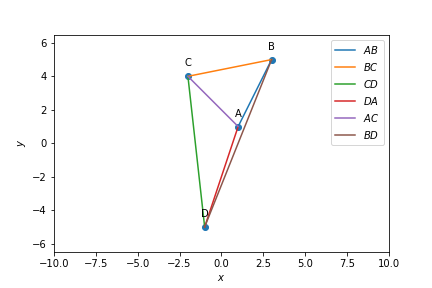
\includegraphics[width=\linewidth]{QUAD.png}
  \caption{Quadrilateral ABCD}
  \label{fig:graph1}
\end{figure}
\\
The above figure clearly depicts the other set of points are not collinear. Hence the points given form a Quadrilateral.

\textbf{Using Method-II}:
\\
Area of a Triangle formed by points \myvec{x_1,y_1},\myvec{x_2,y_2},\myvec{x_3,y_3} is given by
\\
\begin{equation}
\begin{math}
\frac{1}{2}
\begin{vmatrix}
x_1 & y_1 & 1\\x_2 & y_2 & 1\\x_3 & y_3 & 1\\
\end{vmatrix}
\end{math}
\end{equation}
\\
Area of Triangle formed by
A\myvec{1,1},B\myvec{3,5},D\myvec{-1,-5} is given by\\
\Delta ABD = 
\begin{math}
\frac{1}{2}
\begin{vmatrix}
1 & 1 & 1\\3 & 5 & 1\\-1 & -5 & 1\\
\end{vmatrix}
\end{math}
= -2\\
\\
Since Area of \Delta ABD $\neq$ 0, the points are non collinear and all other points show a distinct area between the points, it can be ascertained that the points form a Quadrilateral.


\subsection{Area of a Quadrilateral}
\\
Area of a \Box ABCD = \\Area of Triangle \Delta ACD + Area of Triangle \Delta ABC \\

since this does not fall into category of Square, Parallelogram or Rhombus, Trapezium.
\\
\\
Area of Triangle formed by
A\myvec{1,1},B\myvec{3,5},C\myvec{-2,4} is given by\\
\Delta ABD = 
\begin{math}
\frac{1}{2}
\begin{vmatrix}
1 & 1 & 1\\3 & 5 & 1\\-2 & 4 & 1\\
\end{vmatrix}
\end{math}
= 9\\
\\
Area of Triangle formed by
A\myvec{1,1},C\myvec{-2,4},D\myvec{-1,-5} is given by\\
\Delta ABD = 
\begin{math}
\frac{1}{2}
\begin{vmatrix}
1 & 1 & 1\\-2 & 4 & 1\\-1 & -5 & 1\\
\end{vmatrix}
\end{math}
= 11.5\\
\\
\begin{lstlisting}
The area of quadrilateral ABCD = 9+11.5 = 20.5
\end{lstlisting}
\end{document}